%1.1
\setcounter{chapter}{1}
\section{Things you can do with PDF\\PDF的用途}

Let’s start with six quick facts about PDF:\\让我们从六个关于PDF的快速事实开始:

\begin{itemize}
\item
PDF is the Portable Document Format.\\PDF是可移植文档格式。

\item
It’s an open file format (ISO-32000-1), originally created by Adobe.\\它是一个开放的文件格式(ISO-32000-1),最初由Adobe创建。

\item
It’s used for documents that are independent of system software and hardware.\\它用于独立于系统软件和硬件的文档。

\item
PDF documents are an essential part of the web.\\PDF文档是Web的关键部分。

\item
Adobe Reader is the most widely used PDF viewer.\\Adobe Reader是最广泛使用的PDF阅读器。

\item
There are a lot of free and proprietary, open and closed source, desktop and web-based software products for creating, viewing, and manipulating PDF documents.\\有许多免费和专有的、开放和闭源的、桌面和基于Web的软件产品,用于创建、查看和操作PDF文档。
\end{itemize}

Figure \ref{fig:PDF相关功能概述} offers an overview of the things you can do with PDF. There are tools to create PDF documents, there are applications to consume PDF documents, and there are utilities to manipulate existing PDF documents.

图 \ref{fig:PDF相关功能概述} 提供了关于使用PDF所能做的事情的概述。有用于创建PDF文档的工具,有用于消费PDF文档的应用程序,还有用于操作现有PDF文档的实用程序。

% Figure 1.1 Overview of
% PDF-related functionality.
% The functionality covered
% by iText is marked with
% the iText logo.
\begin{myfigure}{PDF相关功能概述。iText涵盖的功能标有iText标志。\label{fig:PDF相关功能概述}}
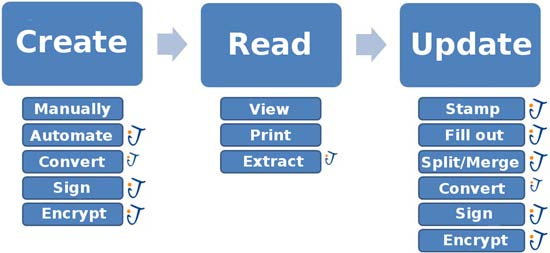
\includegraphics[height=4cm]{/Users/virhuiai/hlProjects/Latex-Typesetting-Hub/练习书本排版/iText_in_Action_Second_Edition/Creating_PDF_documents_from_scratch/Introducing_PDF_and_iText/index-35_1.jpg}
\end{myfigure}

% 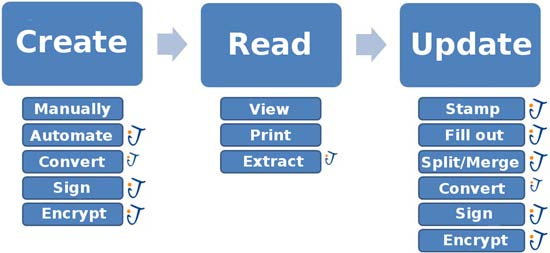
\includegraphics[height=4cm]{/Users/virhuiai/hlProjects/Latex-Typesetting-Hub/练习书本排版/iText_in_Action_Second_Edition/Creating_PDF_documents_from_scratch/Introducing_PDF_and_iText/index-35_1.jpg}

If you look at PDF creation, you’ll find that graphical designers use desktop applications such as Adobe Acrobat or Adobe InDesign to create a document in a manual or semimanual process. In another context, PDF documents are created programmatically, using an API to produce PDFs directly from software applications, without—--or with minimal—human intervention. Sometimes the document is created in an inter-mediary format first, then converted to PDF. These different approaches demand different software products. The same goes for PDF manipulation. You can update a PDF
manually in Adobe Acrobat, but there are also tools that allow forms to be filled out automatically based on information from a database.

如果您看PDF的创建,您会发现图形设计师使用桌面应用程序,如Adobe Acrobat或Adobe InDesign,以手动或半自动的方式创建文档。在另一种情况下,使用API从软件应用程序直接生成PDF,而不需要或只需要最少的人工干预。有时文档首先以中介格式创建,然后转换为PDF。这些不同的方法需要不同的软件产品。对于PDF操纵也是如此。您可以在Adobe Acrobat中手动更新PDF,但也有工具可以根据来自数据库的信息自动填写表格。

This book will focus on the automation side of things: we’ll create and manipulate PDF documents in an automated process using iText. The functionality covered by iText in figure \ref{fig:PDF相关功能概述} is marked with the iText logo. A smaller logo indicates that the functionality is only partly supported.

本书将关注自动化方面:我们将使用iText创建和操作PDF文档的自动化过程。图 \ref{fig:PDF相关功能概述} 中iText所涵盖的功能都被标记有iText的标志。较小的标志表示该功能仅部分支持。

Typically, iText is used in projects that have one of the following requirements:

通常,iText在具有以下要求的项目中使用:

\begin{itemize}
\item
The content isn’t available in advance: it’s calculated based on user input or real-time database information.

内容事先不可用:它是基于用户输入或实时数据库信息进行计算的。

\item
The PDF files can’t be produced manually due to the massive volume of content: a large number of pages or documents.

由于内容数量庞大(大量页面或文档),无法手动生产PDF文件。

\item
Documents need to be created in unattended mode, in a batch process.

需要在批处理过程中以无人值守模式创建文档。

\item
The content needs to be customized or personalized; for instance, the name of the end user has to be stamped on a number of pages.

需要自定义或个性化内容;例如,必须在多个页面上盖上最终用户的名称。
\end{itemize}
Often you’ll encounter these requirements in web applications, where content needs to be served dynamically to a browser. Normally, you’d serve this information in the form of HTML, but for some documents, PDF is preferred over HTML for better printing quality, for identical presentation on a variety of platforms, for security reasons, or to reduce the file size. In this case, you can serve PDF on the fly.

通常,您会在Web应用程序中遇到这些要求,在这些应用程序中,需要动态地向浏览器提供内容。通常情况下,您会以HTML的形式提供此信息,但是对于某些文档,出于更好的打印质量、在各种平台上相同的展示效果、出于安全原因或减小文件大小等原因,PDF优于HTML。这种情况下,您可以实时提供PDF。

As you read this book, you’ll create and manipulate hundreds of PDF documents that demonstrate how to use a specific feature, how to solve common and less common issues, and how to build an application that involves PDF technology. We’ll use iText because it’s an API that was developed to allow developers to do the following (and much more):

在阅读本书时,您将创建和操作数百个PDF文档,演示如何使用特定功能,如何解决常见和不常见的问题以及如何构建涉及PDF技术的应用程序。我们将使用iText,因为它提供的API,旨在使开发人员能够执行以下操作(以及更多操作):
\begin{itemize}
\item
Generate documents and reports based on data from an XML file or a database

基于XML文件或数据库中的数据生成文档和报告

\item
Create maps and books, exploiting numerous interactive features available in PDF

创建地图和书籍,利用PDF中众多交互功能
\item
Add bookmarks, page numbers, watermarks, and other features to existing PDF
documents

向现有PDF文档添加书签、页码、水印和其他功能

\item
Split or concatenate pages from existing PDF files

从现有的PDF文件中拆分或连接页面
\item
Fill out interactive forms

填写交互式表单
\item
Serve dynamically generated or manipulated PDF documents to a web browser 

向Web浏览器提供动态生成的或操作过的PDF文档
\end{itemize}
For first-time users, this book is indispensable. Although the basic functionality of iText is easy to grasp, the first parts of this book significantly lower the learning curve and gradually offer more advanced functionality.

对于首次使用者,本书是必不可少的。虽然iText的基本功能易于掌握,但是本书的前几部分显着降低了学习曲线,并逐渐提供更高级的功能。

It’s also a must-have for the many developers who are already familiar with iText.

对于已经熟悉iText的许多开发人员来说,这也是必备的。

In the final chapters, many PDF secrets hidden in ISO-32000-1, the open standard that defines the Portable Document Format, will be unveiled. Even experienced iText developers will learn new ways to master the PDF specification using their favorite PDF library.

在最后几章中,将揭示隐藏在ISO-32000-1中的许多PDF机密,该开放标准定义了可移植文档格式。即使是经验丰富的iText开发人员也将学习使用他们喜欢的PDF库来掌握PDF规范的新方法。

Without further ado, let’s start with a simple example that explains how to compile and run the many examples that come with this book.

言归正传,让我们从一个简单的示例开始,解释如何编译和运行本书中包含的许多示例。


%%%%%%%% 以下跳过
% 翻译成中文:1.2

% Working with the examples in this book

% All the source files, as well as the resources and extra libraries necessary to run the book’s examples, were uploaded to a Subversion (SVN) repository on SourceForge. If you have an SVN client, you can check out of the complete working environment at once. This way, you’ll be able to get the latest updates and new examples, even after the book has been released. Please consult appendix B for the URL of this repository.

% You can find more info about this on the examples page of the itextpdf.com site.

% That’s also the place where you’ll find zipped archives, in case you don’t have an SVN

% client. You can download these archives and unzip them on your local system.

% Before you start experimenting, make sure that you have a recent version of the Java Development Kit (JDK) installed. The examples won’t work for versions of iText that are older than iText 5, and iText 5 is compiled with Java 5, so the minimum requirement for your JVM is Sun’s JDK 1.5. You can use other JDKs, but only the JDK

% from Sun is supported.

% Figure 1.2 shows how I compiled and executed the first example, HelloWorld, on Ubuntu Linux using OpenJDK 6. As you can see, you first change the directory to the examples folder (or whichever folder contains your copy of the project). Then you run this command:

% javac -d bin -cp lib/iText.jar src/part1/chapter01/HelloWorld.java HelloWorld.java is the source file; we’ll take a close look at it in the next section. The option -d says that the compiled code should be written to the bin folder. With option

% -cp you define the classpath. For this simple example, you only need the iText.jar file.

% For other examples, you might need to add more JARs, such as a JAR with the database driver, encryption JARs, and so forth.

% Once you’ve compiled the code, you can execute it:

% java -cp "bin:lib/iText.jar" part1.chapter01.HelloWorld

% If you’re working on Windows, you’ll need to replace the colon separating the different parts of the classpath with a semicolon:

% java -cp "bin;lib/iText.jar" part1.chapter01.HelloWorld

% Congratulations! You have created your first PDF file using iText. Figure 1.3 shows how everything is organized.

% The source code of the examples can be found in the src folder; see, for instance, the file HelloWorld.java. The package names of the examples correspond to the part and chapter numbers of the book. In the lib directory, you’ll find all the JARs you Figure 1.2 Compiling and running from the command line





% Working with the examples in this book

% 7

% Figure 1.3 Organization of the sample files

% need to compile the examples. There’s also a resources folder containing all the resources you might need to run the examples: database scripts, images, special fonts, and existing PDF files, such as interactive forms.

% The examples are compiled to the bin folder. The HelloWorld.class file will appear as soon as you run the javac command. When you execute the java command, you’ll see the hello.pdf file appear in the results directory. Figure 1.4 shows the end result: a PDF file containing the text “Hello World!”

% It’s certainly possible to compile and execute all the examples from the command line, but it’s more likely that you’ll prefer using an integrated development environment (IDE). Figure 1.5 shows what the project looks like in Eclipse—you’ll recognize the same folders. Observe that Eclipse puts the src folder on top. The bin directory is hidden; you’ll find the JARs under Referenced Libraries. You can view and update the list of registered JARs by selecting Project > Properties > Java Build Path > Libraries.

% Figure 1.4

% A “Hello World” PDF



% 8

% CHAPTER 1 Introducing PDF and iText

% Figure 1.5 The project opened in Eclipse

% Figure 1.5 already gives you a peek at the source code. The hello.pdf file is created in five steps. The next section discusses every step in detail.


%%%%%%%%跳过的翻译
% 在本书中使用示例

% 所有的源文件以及运行本书示例所需的资源和额外的库都上传到了SourceForge的Subversion(SVN)仓库中。如果您有一个SVN客户端,您可以一次性检出完整的工作环境。这样,即使在本书发布后,您也能够获得最新的更新和新的示例。请参阅附录B获取此仓库的URL。

% 您可以在itextpdf.com网站的示例页面上找到更多信息。

% 那里也是您可以找到压缩的存档文件的地方,以防您没有SVN客户端。您可以下载这些存档文件并在本地系统上解压缩。

% 在开始实验之前,请确保您安装了最新版本的Java开发工具包(JDK)。示例不适用于早于iText 5的iText版本,并且iText 5是使用Java 5编译的,因此您的JVM的最小要求是Sun的JDK 1.5。您可以使用其他JDK,但仅支持Sun的JDK。

% 图1.2显示了我如何在Ubuntu Linux上使用OpenJDK 6编译和执行第一个示例HelloWorld。您可以看到,您首先要将目录更改为示例文件夹(或包含项目副本的任何文件夹)。然后运行此命令:

% javac -d bin -cp lib/iText.jar src/part1/chapter01/HelloWorld.java

% HelloWorld.java是源文件;我们将在下一节中仔细查看它。选项-d表示编译代码应写入bin文件夹。使用选项-cp定义类路径。对于这个简单的示例,您只需要iText.jar文件。

% 对于其他示例,您可能需要添加更多的JAR,例如具有数据库驱动程序、加密JAR等的JAR。

% 一旦您编译了代码,就可以执行它:

% java -cp "bin:lib/iText.jar" part1.chapter01.HelloWorld

% 如果您正在Windows上工作,则需要用分号替换类路径中不同部分之间的冒号:

% java -cp "bin;lib/iText.jar" part1.chapter01.HelloWorld

% 恭喜!您已经使用iText创建了您的第一个PDF文件。图1.3显示了所有内容的组织方式。

% 示例的源代码可以在src文件夹中找到;例如,参见文件HelloWorld.java。示例的包名称与书的部分和章节编号相对应。在lib目录中,您会找到编译示例所需的所有JAR。还有一个资源文件夹,其中包含运行示例所需的所有资源:数据库脚本、图像、特殊字体以及现有的PDF文件,例如交互式表单。

% 示例编译到bin文件夹。当您运行javac命令时,HelloWorld.class文件将立即出现。当您执行java命令时,您将在results目录中看到hello.pdf文件出现。图1.4显示了最终结果:包含文本“Hello World!”的PDF文件。

% 当然,可以通过命令行编译和执行所有示例,但更可能的是您会更喜欢使用集成开发环境(IDE)。图1.5显示了在Eclipse中打开项目的情况——您会认出相同的文件夹。请注意,Eclipse将src文件夹置于顶部。bin目录被隐藏起来;您将在引用库下找到JAR。您可以通过选择Project > Properties > Java Build Path > Libraries来查看和更新注册JAR的列表。

% 图1.5已经为您展示了源代码的一瞥。hello.pdf文件是通过以下五个步骤创建的。下一节将详细讨论每个步骤。